\section{Topic 4. Numerical Differentiation and Integration}
We will approximate the derivative $\mathbf{D}_f$ and the integral $\mathbf{I}_f$ of a real-valued function $f: \R \rightarrow \R$ restricted to $[a,b]$. Recall that,
\[\mathbf{D}(f)(x_0) = \lim _{h \rightarrow 0} \frac{f\left(x_0+h\right)-f\left(x_0\right)}{h}
\]
for every point $x_0 \in [a, b]$. In this way, $\mathbf{D}(f)(x_0)$ is said to be determined by \textbf{local information} about $f$ around $x_0$. In contrast,
\[\mathbf{I}_f |_a^b = \lim _{n \rightarrow \infty} \sum_{i=1}^n f\left(x_i\right) \Delta x\quad \text{ where } \quad \Delta x := \frac{b-a}{n}\]
is determined by \textbf{global information} about $f$ on $[a, b]$.

\begin{marginfigure}
    We will use the following notation,
    \begin{align*}
        &\mathbf{D}(f) := \text{ exact derivative of } f \\
        &\mathbf{D}_h(f) := \text{ approximate derivative of } f \\
        &\mathbf{I}(f) := \text{ exact integral of } f \\
        &\mathbf{I}_h(f) := \text{ approximate integral of } f \\
    \end{align*}
\end{marginfigure}

\begin{defn}[Degree of Accuracy]
    We say that,
    \sloppy \begin{enumerate}
        \item $\mathbf{D}_h(f)$ has \textbf{degree of accuracy} of $p$ if $p$ is the largest positive integer with \text{$\mathbf{D}(x^i) = \mathbf{D}_h (x^i)$} for any $x$ and \text{$i = 0, \cdots p$}
        \item $\mathbf{I}_h(f)$ has \textbf{degree of accuracy} of $p$ if $p$ is the largest positive integer with \text{$\mathbf{I}(x^i) = \mathbf{I}_h (x^i)$} for any $x$ and \text{$i = 0, \cdots p$}
    \end{enumerate}
\end{defn}

\subsection{Numerical Differentiation}
The simplest method for approximating $\mathbf{D}(f)$ is to use Taylor's remainder theorem. Define a partition of the interval $[a,b]$ using
\[x_k = a + kh \quad \text{where} \quad h := \frac{b-a}{n}\]
and expand $f$ about $x_k$. There exists $\xi(x) \in (x, x_k)$ such that,
\[f(x) = f(x_k) + f^{\prime}(x_k)(x-x_k) + \frac{f^{\prime\prime}(\xi(x))}{2}(x-x_k)^2\]
Setting $x = x_{k+1}$ gives that,
\[f\left(x_{k+1}\right)=f\left(x_k\right)+f^{\prime}\left(x_k\right) h+\frac{f^{\prime \prime}\left(\xi\left(x_{k+1}\right)\right)}{2} h^2\]
which we can re-arrange to obtain,
\[\underbrace{f^{\prime}\left(x_k\right)}_{\mathbf{D} (f\left(x_k\right))}=\underbrace{\frac{f\left(x_{k+1}\right)-f\left(x_k\right)}{h}}_{\mathbf{D}_h (f\left(x_k\right))}+\underbrace{\frac{-f^{\prime \prime}\left(\xi\left(x_{k+1}\right)\right)}{2} h}_{\mathcal{O}(h)}\]
From this, we obtain the \textbf{forward difference formula}. Similarly, the\textbf{backward difference formula} is obtained by setting $x = x_{k - 1}$.

\begin{marginfigure}
\begin{center}
       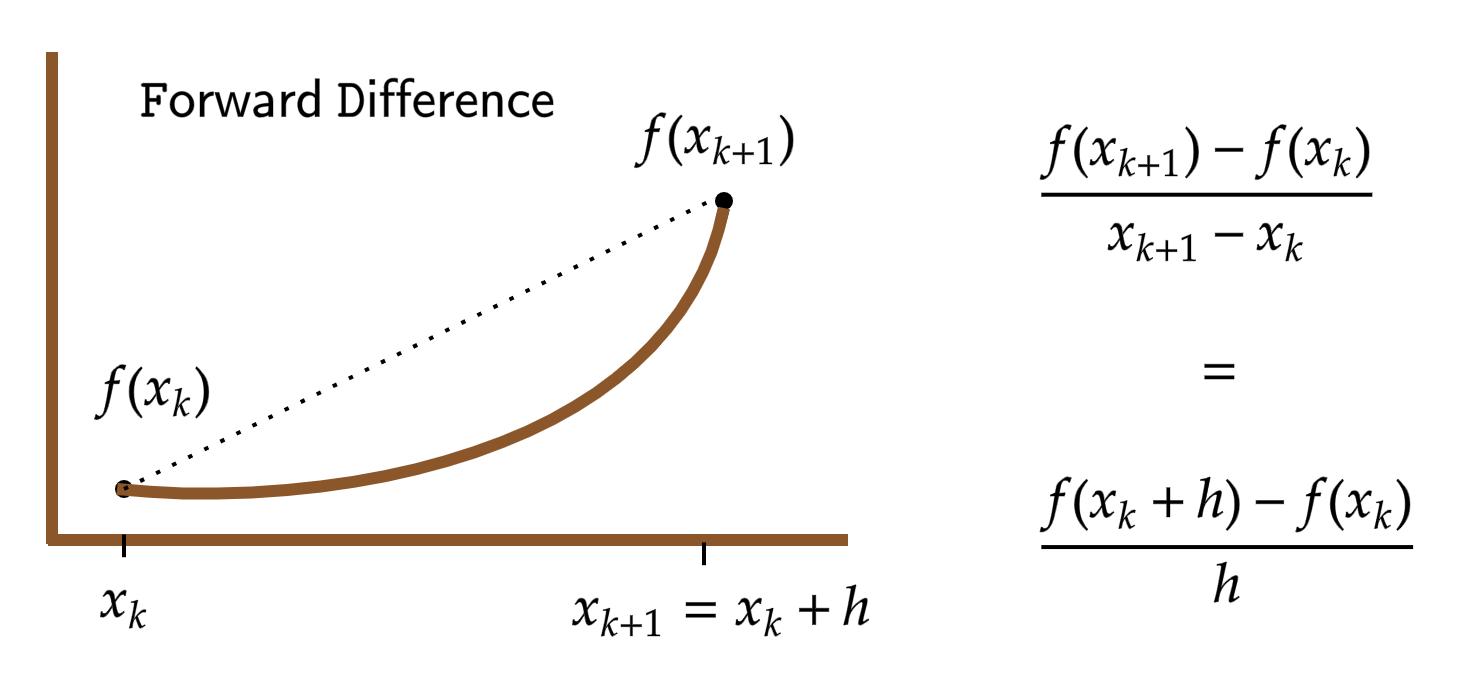
\includegraphics[width=\textwidth]{figures/fig-22.png}
\end{center}
\end{marginfigure}

\begin{defn}[Forward Difference]
    The \textbf{forward difference} is,
    \[\mathbf{D}_h (f(x_k)) := \frac{f(x_{k+1}) - f(x_k)}{h}\]
\end{defn}

\begin{defn}[Backward Difference]
    The \textbf{backward difference} is,
    \[\mathbf{D}_h (f(x_k)) := \frac{f(x_{k}) - f(x_{k-1})}{h}\]
\end{defn}

\NewLine

\noindent The error term that we derived
\[-\frac{h}{2} \cdot f^{\prime \prime}\left(\xi\left(x_{k+1}\right)\right)\]
is proportional to $f^{\prime\prime}$. This implies that $\mathbf{D}_h(f(x^i))$ is exact for $i \in \{0, 1\}$, that is, has a degree of accuracy of $1$.

\NewLine

\begin{defn}[Second Derivative Central Difference]
    We define,
    \[\mathbf{D}^2_h (f(x_k)) := \frac{f\left(x_{k+1}\right)-2 f\left(x_k\right)+f\left(x_{k-1}\right)}{h^2}\]
    as the \textbf{second derivative central difference}.
\end{defn}

\NewLine

\noindent We expand $f$ up to the fourth order using Taylor's Theorem around $x_k$. This gives the \textbf{second derivative central difference},
\begin{align*}
f(x)=& f\left(x_k\right)+f^{\prime}\left(x_k\right)\left(x-x_k\right)+\frac{f^{\prime \prime}\left(x_k\right)}{2}\left(x-x_k\right)^2 \\
&+\frac{f^{(3)}\left(x_k\right)}{3 !}\left(x-x_k\right)^3+\frac{f^{(4)}(\xi(x))}{4 !}\left(x-x_k\right)^4
\end{align*}
Evaluating $f$ at $x = x_{k+1}$ gives,
\[f\left(x_{k+1}\right)=f\left(x_k\right)+f^{\prime}\left(x_k\right) h+\frac{f^{\prime \prime}\left(x_k\right)}{2} h^2+\frac{f^{(3)}\left(x_k\right)}{3 !} h^3+\frac{f^{(4)}\left(\xi\left(x_{k+1}\right)\right)}{4 !} h^4\]
Evaluating $f$ at $x = x_{k-1}$ gives,
\[f\left(x_{k-1}\right)=f\left(x_k\right)-f^{\prime}\left(x_k\right) h+\frac{f^{\prime \prime}\left(x_k\right)}{2} h^2-\frac{f^{(3)}\left(x_k\right)}{3 !} h^3+\frac{f^{(4)}\left(\xi\left(x_{k-1}\right)\right)}{4 !} h^4\]
Adding these two formulas and re-arranging gives,
\begin{align*}
    \underbrace{f^{\prime \prime}\left(x_k\right)}_{\mathbf{D}^2 (f\left(x_k\right))}
    &=\underbrace{\frac{f\left(x_{k+1}\right)-2 f\left(x_k\right)+f\left(x_{k-1}\right)}{h^2}}_{\mathbf{D}_h^2 (f\left(x_k\right))} \\
    &-\underbrace{\frac{f^{(4)}\left(\xi\left(x_{k+1}\right)\right)+f^{(4)}\left(\xi\left(x_{k-1}\right)\right)}{4 !} h^2}_{\mathcal{O}\left(h^2\right)}
\end{align*}

\begin{marginfigure}
    Expanding $f$ up the third order would have given an $\mathcal{O}\left(h\right)$ error term.
\end{marginfigure}

\noindent The error term that we derived is proportional to $f^{(4)}$. This implies that $\mathbf{D}^2_h(f(x^i))$ is exact for $i \in \{0, 1, 2, 3\}$, that is, has a degree of accuracy of $3$. We can simplify the error term as follows,

\begin{rmk}
    There exists $\xi_k$ between $\xi(x_{k-1})$ and $\xi(x_{k+1})$ so that,
    \[f^{(4)}\left(\xi_k\right)=\frac{f^{(4)}\left(\xi\left(x_{k+1}\right)\right)+f^{(4)}\left(\xi\left(x_{k-1}\right)\right)}{2}\]
\end{rmk}

\begin{proof}
    Apply the Intermediate Value Theorem.
\end{proof}

\NewLine 

We want to design more accurate finite difference approximations. Our current approximation schemes are a linear combination of the function values $f(x_{k-1}), f(x_k), f(x_{k+1})$. The natural extension is to use more function values at different points:
\[\mathbf{D}_h (f(x_k)) = \sum_{i=-L}^R a_i \cdot f(x_{k+i})\]
where the neighbouring points $x_{k+i}$ of $x_k$ form the \textbf{stencil} of $\mathbf{D}_h(f)$. The constants $a_i$ are the coefficients associated with the stencil. We will derive the finite difference approximation for $\mathbf{D}(f)$ using
\[\mathbf{D}_h f(x)=a f(x+h)+b f(x)+c f(x-h)\]
and maximizing for degree of accuracy. There are three parameters, $a$, $b$, and $c$, so we can achieve a degree of accuracy of two.
\[0=\mathbf{D}(1)=\mathbf{D}_h(1)=a+b+c \Rightarrow a+b+c=0\]
Next, we have that,
\begin{align*}
1=\mathbf{D}(x) &=\mathbf{D}_h(x)=a(x+h)+b x+c(x-h) \\
&=\underbrace{(a+b+c)}_{=0} x+(a-c) h \Rightarrow a-c=\frac{1}{h}
\end{align*}
Finally,
\begin{align*}
2 x=\mathbf{D}(x^2) &=\mathbf{D}_h(x^2)=a(x+h)^2+b x^2+c(x-h)^2 \\
&=\underbrace{(a+b+c)}_{=0} x^2+\underbrace{(a-c) h}_1 \cdot 2 x+(a+c) h^2 \\
&\Rightarrow a+c=0
\end{align*}
This gives the \textbf{central difference} formula,
\[\mathbf{D}_h (f(x)) := \frac{f(x+h)-f(x-h)}{2 h}\]
which has a degree of accuracy of $2$. Expand using Taylor's Theorem around $x$ and evaluate $x + h$ and $x - h$. For some $\xi^{\pm} \in (x, x \pm h)$,
    \begin{align*}
    &f(x+h)=f(x)+f^{\prime}(x) h+\frac{f^{\prime \prime}(x)}{2} h^2+\frac{f^{(3)}\left(\xi^{+}\right)}{3 !} h^3 \\
    &f(x-h)=f(x)-f^{\prime}(x) h+\frac{f^{\prime \prime}(x)}{2} h^2-\frac{f^{(3)}\left(\xi^{-}\right)}{3 !} h^3
    \end{align*}
    Subtracting these two equations and re-arranging gives,
    \[\underbrace{f^{\prime}(x)}_{\mathbf{D} f(x)}=\underbrace{\frac{f(x+h)-f(x-h)}{2 h}}_{\mathbf{D}_h f(x)}+\underbrace{\frac{f^{(3)}\left(\xi^{+}\right)+f^{(3)}\left(\xi^{-}\right)}{12} h^2}_{\mathcal{O}\left(h^2\right)}\]
    which we can simplify by the Intermediate Value Theorem to,
    \[\frac{h^2}{6} \cdot f^{(3)}(\xi(x))\]

    \begin{ex}{Caveat in Numerical Differentiation}{label}
        Consider the central difference approximation $\mathbf{D}_h (f(x))$ for,
        \[f(x) = \sin(x)\]

        \begin{center}
            \begin{tabular}{|c|c|}
            \hline$h$ & $\left|\mathbf{D} f(\pi)-\mathbf{D}_h f(\pi)\right|$ \\
            \hline $10^0$ & $0.158529015192104$ \\
            $10^{-1}$ & $0.00166583353171768$ \\
            $10^{-2}$ & $1.66665833548629 \mathrm{e}-05$ \\
            $10^{-3}$ & $1.66666768497414 \mathrm{e}-07$ \\
            $10^{-4}$ & $1.66455649264208 \mathrm{e}-09$ \\
            $10^{-5}$ & $1.01152419773598 \mathrm{e}-11$ \\
            $10^{-6}$ & $1.39611433525033 \mathrm{e}-10$ \\
            $10^{-7}$ & $1.63658042673376 \mathrm{e}-09$ \\
            $\vdots$ & $\vdots$ \\
            $10^{-12}$ & $8.89005823410116 \mathrm{e}-05$ \\
            \hline
            \end{tabular}
        \end{center}

        \NewLine 
        
        Errors that occur when computing $f(x + h)$ and $f(x-h)$ are amplified by the division by $h$ because $h$ tends to $\epsilon_{\operatorname{mach}}$.
    \end{ex}

\noindent Due to round-off and discretization, $\tilde{f}$ approximates $f$ up to $\epsilon$.
    \begin{align*}
    &|\tilde{f}(x+h)-f(x+h)| \leq \epsilon \\
    &|\tilde{f}(x-h)-f(x-h)| \leq \epsilon
\end{align*}
Therefore, the actual error can be estimated in three parts,
\begin{align*}
\left|f^{\prime}(x)-\mathbf{D}_h \tilde{f}(x)\right|&=\left|f^{\prime}(x)-\frac{\tilde{f}(x+h)-\tilde{f}(x-h)}{2 h}\right| \\
&=\left|\left(f^{\prime}(x)-\frac{f(x+h)-f(x-h)}{2 h}\right)\right. \\
&\quad \quad +\left.\left(\frac{f(x+h)-\tilde{f}(x+h)}{2 h}\right)+\left(\frac{\tilde{f}(x-h)-f(x-h)}{2 h}\right) \right| \\
&\leq\left|\frac{f^{(3)}(\xi(x))}{3 !} \cdot h^2\right|+\frac{\epsilon}{2 h}+\frac{\epsilon}{2 h} \\
&\leq \frac{M_3}{6} \cdot h^2+\frac{\epsilon}{h} \nrightarrow 0 \text { as } h \rightarrow 0
\end{align*}
by applying the triangle inequality. We want to determine how small $h$ can be before the error dominates. Applying standard results from single-variable calculus, it is left as an exercise to show that
\[\frac{M_3}{6} \cdot h^2+\frac{\epsilon}{h}\]
is minimized at the point,
\[h^*=\left(\frac{3 \epsilon}{M_3}\right)^{\frac{1}{3}}\]

\noindent In summary,
\[\begin{array}{|c|c|c|}
\hline \text { Finite Difference Method } & \text { Error } & \text { Degree of Accuracy } \\
\hline \hline \text { Forward and Backward Difference } & \mathcal{O}(h) & 1 \\
\hline \text { Central Difference } & \mathcal{O}\left(h^2\right) & 2 \\
\hline \text { Second Derivative Central Difference } & \mathcal{O}\left(h^2\right) & 3 \\
\hline
\end{array}\]